\null\newpage
\section{Tieftöner-Verstärker}\label{sec:4.4}
\subsection{Allgemeines}\label{subsec:4.4.1}
Nach dem Filtern des Signals soll dieses vor dem Abstrahlen am Lautsprecher verstärkt werden. Es wurde eine analoge Verstärker-Schaltung verwendet, da diese einfacher und mit weniger Problemen realisiert werden konnte. Mithilfe bereits bekannter, bewährter Schaltungen konnte ein Layout für diese Schaltung designet werden. Ein wichtiger Baustein in dieser Schaltung ist der Verstärker \enquote{TDA2030}, wie in Kapitel \ref{sec:3.2} beschrieben.  Des weiteren wurden zwei Leistungstransistoren verbaut die höhere Ströme schalten können, falls der maximale Schaltstrom des TDA2030 erreicht wird.

\subsection{Zielsetzung}\label{subsec:4.4.2}
Das Eingangssignal soll verstärkt werden um am Ausgang der Schaltung höhere Spannungs-Amplituden und höheren Ströme aufzuweisen. Es soll nach diesem Schritt möglich sein den Tieftöner in einer der zwei Satellitenboxen mit ausreichend Signal zu versorgen, um einen Schalldruck von zumindest Zimmerlautstärke zu erhalten. 

\subsection{Schaltung}\label{subsec:4.4.3}
Leicht ersichtlich in der Schaltung (\ref{fig:4.4.3.1}) ist in der oberen, linken Ecke des Bildes ein Spannungsteiler gegen den Einseranschluss des TDA2030.
Dieser Spannungsteiler, bestehend aus einem Widerstandsnetzwerk, erzeugt den benötigten Arbeitspunkt für die asymmetrische Versorgung des TDA2030.
Mit Hilfe des ELKO's \enquote{EL504} wird verschleppte Gleichspannung am Eingang der Schaltung heraus gesiebt.
Dafür ist auch der ELKO \enquote{EL502}, dieser siebt die Gleichspannung am Ausgang der Schaltung heraus, bevor das Signal den Print verlässt. \\
Über die Widerstände \enquote{R506} und \enquote{R505} wird die Verstärkung der Schaltung eingestellt.
In diesem Fall ist die Verstärkung $\frac{R505+R506}{R505}$ = 31 .
Das bedeutet, dass das Eingangssignal am Ausgang 31mal so groß sein soll, natürlich unter Beachtung der Grenzen der OPV-Verstärkerschaltung(\ref{sec:3.5}).

\begin{figure} [H]
	\centering	
	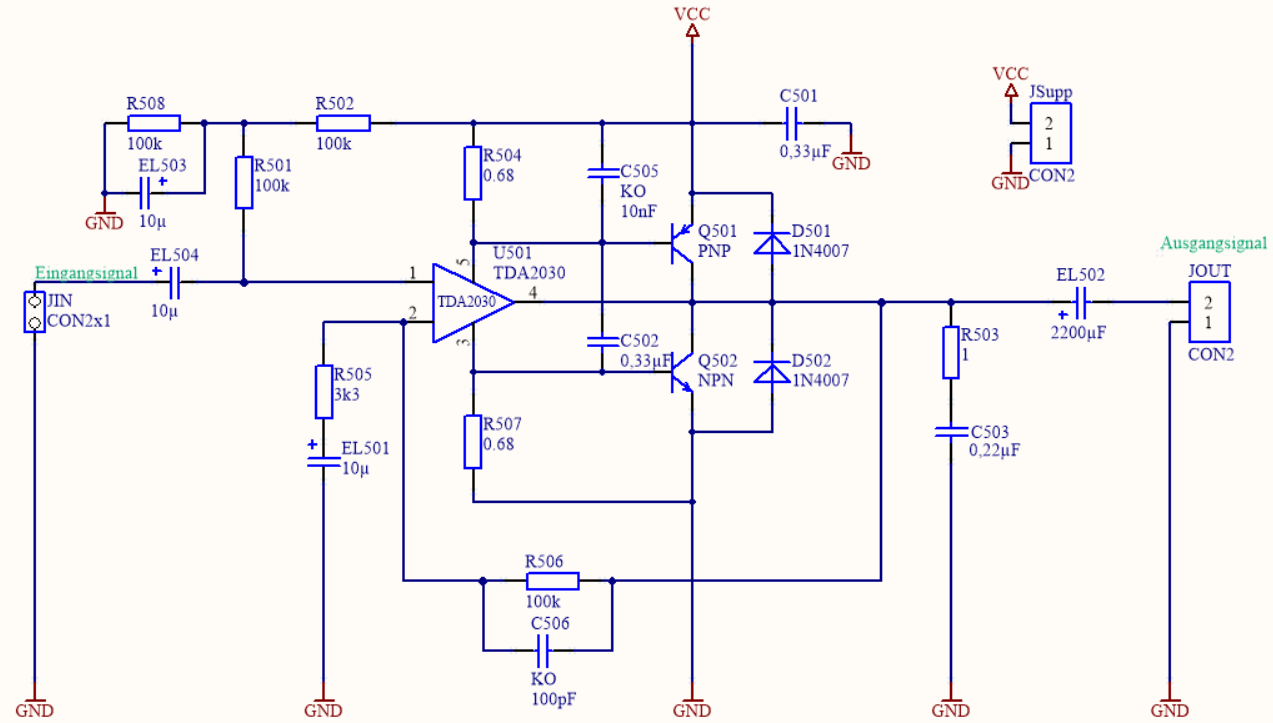
\includegraphics[width=1\textwidth]{img/Print5/5_TTVerstaerker-Schem.PNG}
	\caption{Tieftöner-Verstärker Schaltung}
	\label {fig:4.4.3.1}
\end{figure}

\subsection{PCB}\label{subsec:4.4.4}
Die drei zu kühlenden Bauteile \enquote{Q502, U501, Q501}(\ref{fig:4.4.4.1}) sind auf selber Höhe montiert um sie auf einen Kühlkörper montieren können.
\emph{Zu beachten dabei ist deren Potential an der Kühlfläche!}
Das Potential ist das Selbe wie an dem mittleren Pin.
Daher:
\begin{itemize}
	\item TDA2030: \enquote{-Vcc} = Masse bei asymmetrische Versorgung
	\item PNP(Q501): \enquote{Kollektor} = Ausgangssignal TDA2030
	\item NPN(Q502): \enquote{Kollektor} = Ausgangssignal TDA2030
\end{itemize}

Aus diesem Grund müssen zumindest die zwei Transistoren isoliert am Kühlkörper angebracht werden.\\
Die Ein- und Ausgänge sind wieder auf einer Seite montiert. 
Einheitlich mit dem Hochtönerverstärkerprint(\ref{sec:4.5}) ist von links nach rechts zuerst Versorgungsstecker, dann Eingangssignal und am Ende der Ausgangsstecker.
Ebenso ist Masse jeweils rechts angeordnet um die Einheitlichkeit noch weiter zu erhöhen.\\
Über den zu kühlenden Elementen ist eine große frei Fläche mit Bohrungen um eine bessere mechanische Verbindung mit dem Kühlkörper zu erhalten.
Die vier kleineren Bohrungen waren für einen Testkühlkörper vorgesehen. 
Dieser wurde bald durch einen größeren ersetzt um mehrere Prints montieren zu können.
%Die finale Ausführung ist jedoch nur auf die mechanische Verbindung der Bauteile mit dem Kühlkörper angewiesen.

\begin{figure} [H]
	\centering	
	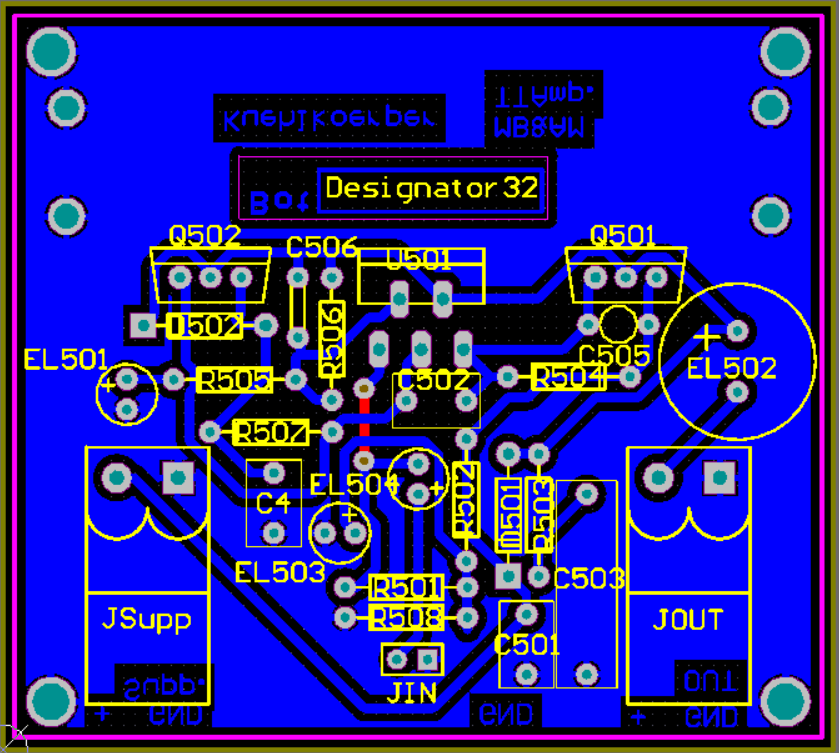
\includegraphics[width=1\textwidth]{img/Print5/5_TTVerstaerker-PCB.PNG}
	\caption{Tieftöner-Verstärker PCB}
	\label {fig:4.4.4.1}
\end{figure}

